\documentclass[12pt,letterpaper]{article}
\usepackage{graphicx,textcomp}
\usepackage{natbib}
\usepackage{graphicx}
\graphicspath{}
\usepackage{setspace}
\usepackage{fullpage}
\usepackage{color}
\usepackage[reqno]{amsmath}
\usepackage{amsthm}
\usepackage{fancyvrb}
\usepackage{amssymb,enumerate}
\usepackage[all]{xy}
\usepackage{endnotes}
\usepackage{lscape}
\newtheorem{com}{Comment}
\usepackage{float}
\usepackage{hyperref}
\newtheorem{lem} {Lemma}
\newtheorem{prop}{Proposition}
\newtheorem{thm}{Theorem}
\newtheorem{defn}{Definition}
\newtheorem{cor}{Corollary}
\newtheorem{obs}{Observation}
\usepackage[compact]{titlesec}
\usepackage{dcolumn}
\usepackage{tikz}
\usetikzlibrary{arrows}
\usepackage{multirow}
\usepackage{xcolor}
\newcolumntype{.}{D{.}{.}{-1}}
\newcolumntype{d}[1]{D{.}{.}{#1}}
\definecolor{light-gray}{gray}{0.65}
\usepackage{url}
\usepackage{listings}
\usepackage{color}

\definecolor{codegreen}{rgb}{0,0.6,0}
\definecolor{codegray}{rgb}{0.5,0.5,0.5}
\definecolor{codepurple}{rgb}{0.58,0,0.82}
\definecolor{backcolour}{rgb}{0.95,0.95,0.92}

\lstdefinestyle{mystyle}{
	backgroundcolor=\color{backcolour},   
	commentstyle=\color{codegreen},
	keywordstyle=\color{magenta},
	numberstyle=\tiny\color{codegray},
	stringstyle=\color{codepurple},
	basicstyle=\footnotesize,
	breakatwhitespace=false,         
	breaklines=true,                 
	captionpos=b,                    
	keepspaces=true,                 
	numbers=left,                    
	numbersep=5pt,                  
	showspaces=false,                
	showstringspaces=false,
	showtabs=false,                  
	tabsize=2
}
\lstset{style=mystyle}
\newcommand{\Sref}[1]{Section~\ref{#1}}
\newtheorem{hyp}{Hypothesis}

\title{Problem Set 1}
\date{Due: September 30, 2024}
\author{Applied Stats/Quant Methods 1}

\begin{document}
	\maketitle
	
	\section*{Instructions}
	\begin{itemize}
	\item Please show your work! You may lose points by simply writing in the answer. If the problem requires you to execute commands in \texttt{R}, please include the code you used to get your answers. Please also include the \texttt{.R} file that contains your code. If you are not sure if work needs to be shown for a particular problem, please ask.
\item Your homework should be submitted electronically on GitHub.
\item This problem set is due before 23:59 on Monday September 30, 2024. No late assignments will be accepted.
%\item Total available points for this homework is 80.
	\end{itemize}
	
	\vspace{1cm}
	\section*{Question 1: Education}

A school counselor was curious about the average of IQ of the students in her school and took a random sample of 25 students' IQ scores. The following is the data set:\\
\vspace{.5cm}

\lstinputlisting[language=R, firstline=36, lastline=36]{PS01_JW.R}  

\vspace{1cm}

\begin{enumerate}
	\item Find a 90\% confidence interval for the average student IQ in the school.\\
\lstinputlisting[language=R, firstline=42, lastline=54]{PS01_JW.R} 

The school counselor conducted a study by taking a random sample of 25 students' IQ scores to estimate the average IQ of all students in the school. After analyzing the data, the sample mean IQ was found to be 98.44.

A 90\% confidence interval was calculated to estimate the range within which the true average IQ of all students in the school is likely to fall.

The 90\% confidence interval for the mean IQ ranges from 94.13 to 102.75. This means that in repeated sampling in 90 out of 100 sample means will fall between 94.13 and 102.75. In other words, we are 90\% confident that the true mean IQ of the students in the school lies between 94.13 and 102.75.\\
	
	\item Next, the school counselor was curious  whether  the average student IQ in her school is higher than the average IQ score (100) among all the schools in the country.\\ 
	
	\noindent Using the same sample, conduct the appropriate hypothesis test with $\alpha=0.05$.
\lstinputlisting[language=R, firstline=55, lastline=58]{PS01_JW.R}  
A one-sample t-test was conducted to determine whether the average IQ of students at a particular school is higher than the national average of 100. The null hypothesis (H0) states that the average IQ of the students is equal to the national average of 100, while the alternative hypothesis (HA) proposed that the average IQ of the students is greater than the national average.

The results yielded a t-value of -0.596 and a p-value of 0.7215, which is greater than the significance level of 0.05. As a result, there is insufficient evidence to reject the null hypothesis. Therefore, it is concluded that the average IQ of students at the school is not significantly higher than the national average. In fact, the sample mean of 98.44 suggests that the average IQ may even be slightly lower, but this difference is not statistically significant.

\end{enumerate}

\newpage

	\section*{Question 2: Political Economy}

\noindent Researchers are curious about what affects the amount of money communities spend on addressing homelessness. The following variables constitute our data set about social welfare expenditures in the USA. \\
\vspace{.5cm}


\begin{tabular}{r|l}
	\texttt{State} &\emph{50 states in US} \\
	\texttt{Y} & \emph{per capita expenditure on shelters/housing assistance in state}\\
	\texttt{X1} &\emph{per capita personal income in state} \\
	\texttt{X2} &  \emph{Number of residents per 100,000 that are "financially insecure" in state}\\
	\texttt{X3} &  \emph{Number of people per thousand residing in urban areas in state} \\
	\texttt{Region} &  \emph{1=Northeast, 2= North Central, 3= South, 4=West} \\
\end{tabular}

\vspace{.5cm}
\noindent Explore the \texttt{expenditure} data set and import data into \texttt{R}.
\vspace{.5cm}
\lstinputlisting[language=R, firstline=54, lastline=54]{PS01_JW.R}  
\vspace{.5cm}
\begin{itemize}

\item
Please plot the relationships among \emph{Y}, \emph{X1}, \emph{X2}, and \emph{X3}? What are the correlations among them (you just need to describe the graph and the relationships among them)?
\lstinputlisting[language=R, firstline=64, lastline=87]{PS01_JW.R} 

\begin{figure}[h]
    \centering
    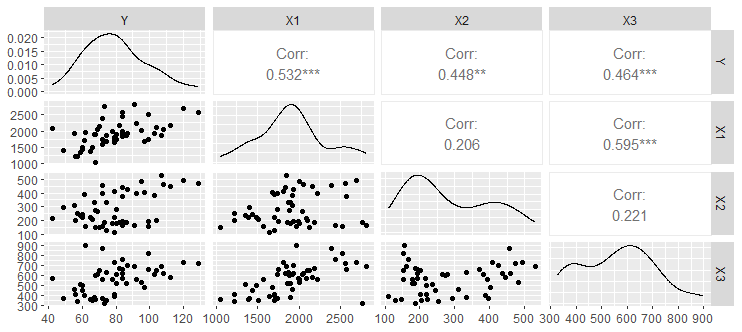
\includegraphics[width=\textwidth]{Rplot07.png}
    \caption{Relationship and Correlation of Variables}
    \label{fig:yourlabel}
\end{figure}

The pair plot shows the relationships among the variables Y (per capita expenditure on housing assistance), X1 (per capita personal income), X2 (number of financially insecure residents), and X3 (urban population). There is a moderate positive correlation between Y and X1 (0.532), indicating that states with higher personal income tend to spend more on housing assistance. Similarly, Y shows a positive correlation with both X2 (0.448) and X3 (0.464), suggesting that states with more financially insecure and urban residents also tend to allocate more towards homelessness expenditures. The strongest relationship is between X1 and X3 (0.595), reflecting that wealthier states generally have larger urban populations. Overall, the data indicate that personal income, urbanization, and financial insecurity are moderately associated with increased housing assistance expenditure.

\vspace{.5cm}
\item
Please plot the relationship between \emph{Y} and \emph{Region}? On average, which region has the highest per capita expenditure on housing assistance
\lstinputlisting[language=R, firstline=90, lastline=101]{PS01_JW.R}  

\begin{figure}[h]
    \centering
    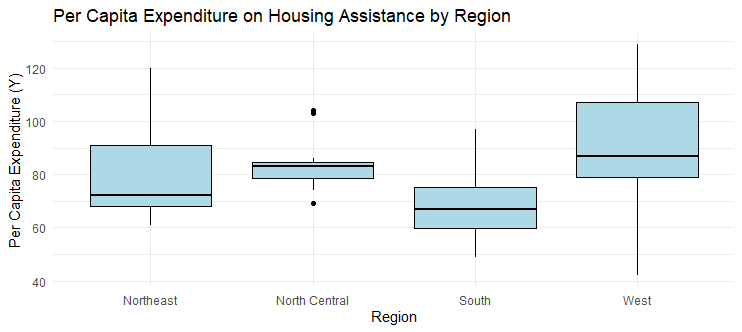
\includegraphics[width=\textwidth]{Boxplot.png}
    \caption{Housing Assistance Expenditure by Region}
    \label{fig:yourlabel}
\end{figure}

The boxplot illustrates the relationship between per capita expenditure on housing assistance (Y) and different regions. The black line inside each box represents the median per capita expenditure for that region, which is the midpoint of the data. The West region has the highest median per capita expenditure, around 90, followed closely by the Northeast, with a median just below 80. The North Central region has a median expenditure of around 78, while the South has the lowest median, around 65. The West also displays the widest range of expenditures, with values ranging from approximately 60 to over 120, indicating significant variability in spending across states in this region. In contrast, the North Central and South regions show much narrower ranges of spending, with the North Central spanning from about 75 to 85. Overall, the West not only has the highest median expenditure but also the greatest variability in per capita spending.


\vspace{.5cm}
\item
Please plot the relationship between \emph{Y} and \emph{X1}? Describe this graph and the relationship. Reproduce the above graph including one more variable \emph{Region} and display different regions with different types of symbols and colors.
\lstinputlisting[language=R, firstline=116, lastline=123]{PS01_JW.R}  

\begin{figure}[h]
    \centering
    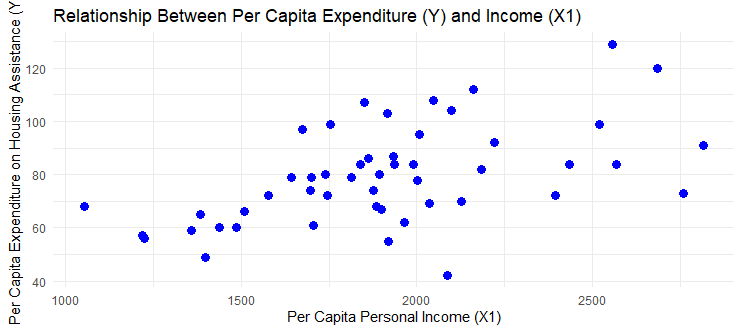
\includegraphics[width=\textwidth]{scatter.png}
    \caption{Relationship of Per Capita Expenditure of Housing Assistance and Per Capita Personal Income}
    \label{fig:yourlabel}
\end{figure}

The scatterplot shows the relationship between per capita personal income (X1) and per capita expenditure on housing assistance (Y). There appears to be a moderate positive correlation between the two variables, as higher personal income is generally associated with higher spending on housing assistance. Most data points are clustered between 1,500USD and 2,000USD for income, with expenditures ranging from 60USD to 100USD. A few outliers exist, with some states showing higher expenditures (up to 120USD) despite varying income levels. Overall, as income increases, there is a tendency for higher housing expenditure, though with some variability.

\lstinputlisting[language=R, firstline=128, lastline=143]{PS01_JW.R}  

\begin{figure}[h]
    \centering
    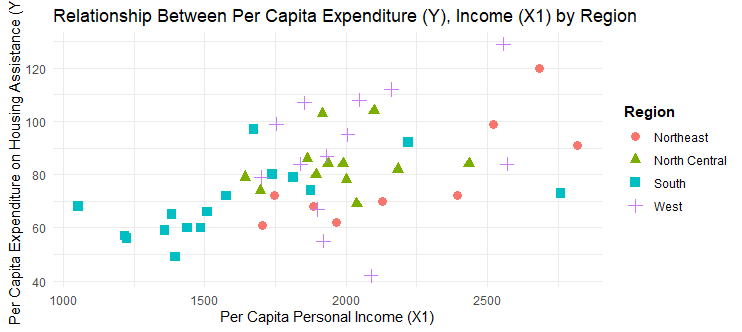
\includegraphics[width=\textwidth]{prettyplot.png}
    \caption{Relationship of Per Capita Expenditure on Housing Assistance and Per Capita Personal Income by Region}
    \label{fig:yourlabel}
\end{figure}

The scatterplot shows a positive relationship between per capita income (X1) and housing expenditure (Y), with regions distinguished by color and shape. The West and Northeast show higher and more variable expenditures, while the South and North Central have lower, more consistent expenditures. Overall, the graph shows again, that higher income is generally associated with greater housing assistance spending, with notable regional differences in variability.

Submitted by Juliane Wesselmann


\end{itemize}


\end{document}
